\documentclass{beamer}
\usepackage{../tut-slides}
\usepackage{../mathoperatorsAuD}

\usepackage{csquotes}
\usepackage{cancel}

\usepackage{amsmath,amssymb}

\usepackage{tikz}

\usetikzlibrary{positioning,automata, matrix, trees, fit}
\usetikzlibrary{calc,backgrounds}
\usetikzlibrary{arrows, arrows.meta}
\usepackage{forest}


\usepackage{booktabs}
\usepackage{tabularx}
\usepackage{tabu}

\renewcommand{\tabularxcolumn}[1]{>{\hspace{0pt}}m{#1}}

\usepackage{listings}
\lstset{ 
	basicstyle=\footnotesize\ttfamily,        % the size of the fonts that are used for the code
	breakatwhitespace=false,         % sets if automatic breaks should only happen at whitespace
	breaklines=true,                 % sets automatic line breaking
	commentstyle=\itshape,    	     % comment style
	escapeinside={\%*}{*)},          % if you want to add LaTeX within your code
	extendedchars=true,              % lets you use non-ASCII characters; for 8-bits encodings only, does not work with UTF-8
	firstnumber=1,                % start line enumeration with line 1000
	frame=none,
	keywordstyle=\bfseries,       % keyword style
	morekeywords={}, 
	language=C,                 % the language of the code
	numbers=left,                    % where to put the line-numbers; possible: (none, left, right)
	numbersep=5pt,                   % how far the line-numbers are from the code
	numberstyle=\tiny\color{cdgray!50}, % the style that is used for the line-numbers
	rulecolor=\color{cddarkblue}, 
	tabsize=2,	                   % sets default tabsize to 2 spaces
}
\lstdefinestyle{am0}{ 
	basicstyle=\footnotesize\ttfamily,        % the size of the fonts that are used for the code
	breakatwhitespace=false,         % sets if automatic breaks should only happen at whitespace
	breaklines=true,                 % sets automatic line breaking
	commentstyle=\color{cdgray},    	     % comment style
	escapeinside={(*@}{@*)},          % if you want to add LaTeX within your code
	extendedchars=true,              % lets you use non-ASCII characters; for 8-bits encodings only, does not work with UTF-8
	firstnumber=1,                % start line enumeration with line 1000
	frame=none,
	keywordstyle=\bfseries,       % keyword style
	morekeywords={READ,LOAD,GT,JMC,STORE,JMP,WRITE}, 
%	language=AM0,                 % the language of the code
	numbers=left,                    % where to put the line-numbers; possible: (none, left, right)
	numbersep=5pt,                   % how far the line-numbers are from the code
	numberstyle=\tiny\ttfamily\color{cdgray!50}, % the style that is used for the line-numbers
	rulecolor=\color{cddarkblue}, 
	tabsize=2,	                   % sets default tabsize to 2 spaces
}


\usepackage{textgreek}


\renewcommand{\emph}[1]{\textbf{#1}}
\newcommand{\coloremph}[1]{\textcolor{cdpurple}{#1}}
\newcommand{\col}[1]{\textcolor{cdpurple}{\boldsymbol{#1}}}
\newcommand{\coll}[1]{\textcolor{cddarkgreen}{\boldsymbol{#1}}}
\newcommand{\colll}[1]{\textcolor{cdorange}{\boldsymbol{#1}}}
%\newcommand{\step}[2][]{\ensuremath{\overset{{#1} (\text{#2})}{=}}}
%\newcommand*{\astep}[2][]{\ensuremath{\overset{{#1} (\text{#2})}&{=}}}

\newcommand{\num}[1]{\ensuremath{\langle #1 \rangle}}

\undef\trans
\DeclareMathOperator{\trans}{trans}

\makeatletter
\let\save@measuring@true\measuring@true
\def\measuring@true{%
	\save@measuring@true
	\def\beamer@sortzero##1{\beamer@ifnextcharospec{\beamer@sortzeroread{##1}}{}}%
	\def\beamer@sortzeroread##1<##2>{}%
	\def\beamer@finalnospec{}%
}
\makeatother

\begin{document}	
	\title{Programmierung}
	\subtitle{Übung 10: C${}_\text{0}$ und abstrakte Maschine AM${}_\text{0}$}
	\author{Eric Kunze}
	\email{eric.kunze@tu-dresden.de}
	\city{TU Dresden}
	\date{22. Juni 2022}
%	\institute{Lehrstuhl für Grundlagen der Programmierung}
	\titlegraphic{
\includegraphics[width=2cm]{../TUD-white.pdf}}
	
	\maketitle
	

%%%%%%%%%%%%%%%%%%%%%%%%%%%%%%%%%%%%%%%%%%%%%%%%%%%%%%%%%%%%%%%%%%%%%%%%%%%%%

\begin{frame}[fragile] \frametitle{Inhalt}
	\begin{enumerate}
		\item Funktionale Programmierung
		\begin{enumerate}
			\item Einführung in Haskell: Listen
			\item Algebraische Datentypen
			\item Funktionen höherer Ordnung
			\item Typpolymorphie \& Unifikation
			\item Beweis von Programmeigenschaften
			\item \textlambda--Kalkül
		\end{enumerate}
		\item Logikprogrammierung
		\item Implementierung einer imperativen Programmiersprache
		\begin{enumerate}
			\item \textbf{Implementierung von C${}_\text{0}$}
			\item Implementierung von C${}_\text{1}$
		\end{enumerate}
		\item Verifikation von Programmeigenschaften
		\item H${}_\text{0}$ -- ein einfacher Kern von Haskell
	\end{enumerate}
\end{frame}



\section{Implementierung von C${}_\text{0}$ und abstrakte Maschine AM${}_\text{0}$}

\begin{frame}[fragile] \frametitle{$C_0$ und $AM_0$}
	\footnotesize
	\begin{itemize}
		\item \textbf{Ziel:} Implementierung einer einfachen Programmiersprache $C_1 \subset C$
		\pause
		\item \emph{Hier:} zunächst Einschränkung auf $C_0 \subset C_1$ 
		\begin{itemize}
			\item genau eine main-Funktion
			\item Zugriff auf \lstinline|stdio| durch \lstinline|#include|	
			\item einzig zugelassende Datenstruktur: \texttt{int}, Konstanten
			\item Kontrollstrukturen: Ein-/Ausgabebefehle, Zuweisungen, Sequenzen, Verzweigungen, bedingte Schleifen
		\end{itemize}
		\pause
		\item \emph{Implementierung} durch
		\begin{itemize}
			\item Syntax von $C_0$
			\item Befehle und Semantik einer abstrakten Maschine $AM_0$
			\item Übersetzer $C_0 \leftrightarrow AM_0$
		\end{itemize}
	\end{itemize}
\end{frame}


\begin{frame} \frametitle{Befehle und Semantik der $AM_0$}
	\footnotesize
	Wir bauen eine abstrakte Maschine $AM_0$, die unsere Berechnungen ausführen kann. Wir benötigen dafür:
	\begin{itemize}
		\item ein Ein- und Ausgabeband,
		\item einen Datenkeller,
		\item einen Hauptspeicher und 
		\item einen Befehlszähler
	\end{itemize}
	Nun müssen aber auch Aktionen ausgeführt werden, wie zum Beispiel das Einlesen vom Eingabeband in den Hauptspeicher. Dafür gibt es folgende Befehle:
\end{frame}

\tikzset{myarrow/.style={-{Stealth[length=3mm, width=2mm, sep=1pt]}, thick}} 
\tikzset{mybackarrow/.style={{Stealth[length=3mm, width=2mm, sep=1pt]}-, thick}} 
\tikzset{mybotharrow/.style={{Stealth[length=3mm, width=2mm, sep=1pt]}-{Stealth[length=3mm, width=2mm, sep=1pt]}, thick}} 
\tikzset{beschriftung/.style={font=\fontsize{15}{0}\selectfont}} 

\newcommand{\befehl}[1]{\textcolor{cdblue}{\texttt{#1}}}

\begin{frame}
	\centering
	\scalebox{0.6}{%
	\begin{tikzpicture}
		\foreach \i in {0,1,2,3} {
			\node[fit={(\i,2) (\i+1,3)}, inner sep=0pt, draw, thick, align=center] (inp\i) {};
			\node[fit={(\i+5,2) (\i+5+1,3)}, inner sep=0pt, draw, thick, align=center] (out\i) {};
			%			\draw[] (\i,2) rectangle ++(1,1) node[pos=.5] (inp\i) {};
			%			\draw[] (\i+5,2) rectangle ++(1,1) node[pos=.5] (out\i) {};
		}
		
		\node[beschriftung, above=0em of inp0.north west, anchor=south west, align=left] (inpText){Input};
		\node[beschriftung, above=0em of out3.north east, anchor=south east, align=right](outText){Output};
		
		% HAUPTSPEICHER
		\foreach \i in {0,...,6} {
			\node[fit={(\i+1,-1) (\i+2,-2)}, inner sep=0pt, draw, thick, align=center] (h\i) {$h.\i$};
			%			\draw[] (\i,-4) rectangle ++(1,1) node[pos=.5] (h\i) {$h.\i$};
		}
		\node[beschriftung, above=0em of h3](HSText){Hauptspeicher};
		%				\draw[arrow,  bend angle=45, bend left] (HSText) -- (4.5,2);
		\draw[mybackarrow] ([xshift=-1em, yshift=1em]h1.north) to[bend left] %
							node[beschriftung, left=2em, anchor=east] (read) {{\onslide<+->{\befehl{READ}}}} %%
							([xshift= 0em, yshift=-1em]inp2.south west);
		\draw[myarrow]     ([xshift= 1em, yshift=1em]h5.north) to[bend right] %
						   node[beschriftung, right=2em] (write) {{\onslide<+->{\befehl{WRITE}}}} %
						   ([xshift= 0em, yshift=-1em]out2.south west);
		
		
		
		% DATENKELLER
		\foreach \i in {1,...,5} {
			\node[fit={(4,-5-\i) (5,-6-\i)}, inner sep=0pt, draw, thick, align=center] (d\i) {$d.\i$};
			%			\draw[red] (rect.east) to[out=0,in=-90] (rect.south);
			%			\draw[] (5,-5 - \i) rectangle ++(-1,-1) node[pos=.5] (d\i) {$d.\i$};
		}
		\draw[thick] ([xshift=-3em]d5.south west) to ([xshift= 3em]d5.south east);
		\node[beschriftung, left=1em of d3, align=right, anchor=east](DKText){Datenkeller};
		
		\draw[mybackarrow] ([xshift=-1em, yshift=1em]d1.north) to[bend left] %
							node[beschriftung, left=2em, anchor=east] (store) {{\onslide<+->{\parbox{1cm}{\befehl{LOAD} \\[.5em] \befehl{LIT}}}}} % 
							([xshift=-1em, yshift=-1em]h3.south);
		\draw[myarrow]     ([xshift= 1em, yshift=1em]d1.north) to[bend right] %
			                 node[beschriftung, right=2em] (load) {{\onslide<+->{\befehl{STORE}}}} %
			                 ([xshift= 1em, yshift=-1em]h3.south);
		
		
		\draw[myarrow] ([xshift= 1em, yshift= 0em]d2.east) to[bend right=120, min distance=3cm] %
		                node[beschriftung, right=1em] (arithmetik) {{\onslide<+->{\parbox{5cm}{\befehl{ADD}, \befehl{MUL}, \befehl{SUB}, \dots \\[.5em] \befehl{EQ}, \befehl{NE}, \befehl{LE}, \befehl{LT}, \dots}}}} %
		                ([xshift= 1em, yshift= 0em]d1.east);
		%		\node[fit={(5,-14) (4, -15)}, inner sep=0pt, draw, thick, align=center] (bz) {$m$};
		%		\node[left=of bz](BZText){Befehlszähler};
		%		
		%		\draw[myarrow]     ([xshift= 1em, yshift=1em]bz.north) to[bend right] ([xshift= 1em, yshift=-1em]d5.south);
		%		\draw[mybackarrow] ([xshift=-1em, yshift=1em]bz.north) to[bend left]  ([xshift=-1em, yshift=-1em]d5.south);
		
		\node[fit={(10,-10) (11, -11)}, inner sep=0pt, draw, thick, align=center] (bz) {$m$};
		\node[beschriftung, above=1em of bz](BZText){Befehlszähler};
		
		\draw[mybotharrow] ([xshift=-1em, yshift= 0em]bz.west) to %
							node[beschriftung, above=0.5em] {{\onslide<+->{\befehl{JMP}}}} %
							node[beschriftung, below=0.5em] {{\onslide<+->{\befehl{JMC}}}} %
							([xshift= 1em, yshift= 0em]d4.east);
		%		\draw[mybackarrow] ([xshift=-1em, yshift=-1em]bz.west) to[bend left]  ([xshift= 1em, yshift=-1em]d3.east);
	\end{tikzpicture}}
\end{frame}

\begin{frame} \frametitle{Semantik der Befehle}
	\footnotesize
	Den Zustand der abstrakten Maschine beschreiben wir durch die Zustände der $5$ Komponenten, also als $5$-Tupel
	\begin{align*}
		&(m,d,h,inp,out)\\
		= \enskip &(\text{Befehlszähler}, \text{Datenkeller}, \text{Hauptspeicher}, \text{Input}, \text{Output})
	\end{align*}
	Jeder Befehl verändert den Zustand der Maschine -- er verändert also die Einträge in diesem Tupel.
	
	\begin{align*}
		\mathcal{C} [\![ \texttt{SUB} ]\!] &(m,d,h,inp,out) \defeq  \\
		&\text{if } d = d.1 : d.2 : \dots : d.n \\
		&\text{then } (m+1, (d.2 - d.1) : d.3 : \dots : d.n, h, inp, out) 
	\end{align*}
\end{frame}

%\begin{frame} \frametitle{Semantik der Befehle}
%	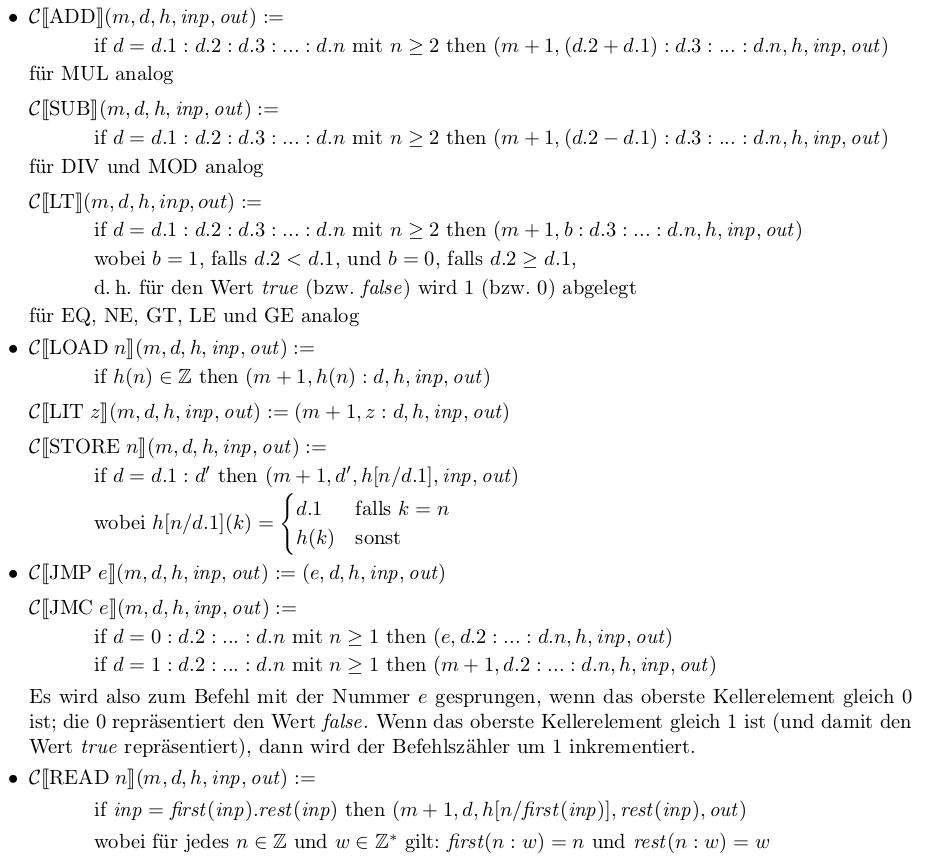
\includegraphics[height=.9\textheight]{tut10-AM0Semantik.jpg} \\
%	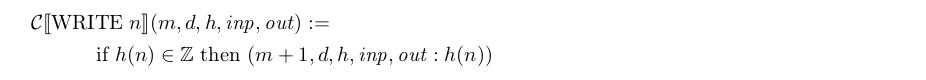
\includegraphics[height=.07\textheight]{tut10-AM0Semantik2.jpg}
%\end{frame}

\begin{frame} \frametitle{Semantik der Befehle -- Arithmetik}
	\small
	\begin{align*}
		\mathcal{C} [\![ \texttt{ADD} ]\!] &(m,d,h,inp,out) \defeq  \\
		&\text{if } d = d.1 : d.2 : \dots : d.n \\
		&\text{then } (m+1, (d.2 + d.1) : d.3 : \dots : d.n, h, inp, out) \\ 
		\tag{analog dazu auch \texttt{MUL}, \texttt{SUB}, \texttt{DIV}, \texttt{MOD}} \\ \pause
		%
		\mathcal{C} [\![ \texttt{LT} ]\!] &(m,d,h,inp,out) \defeq  \\
		&\text{if } d = d.1 : d.2 : \dots : d.n \\
		&\text{then } (m+1, b : d.3 : \dots : d.n, h, inp, out) \\
		&\phantom{\text{then }} \text{wobei } b = 1 \text{ falls } d.2 < d.1 \text{ und } b = 0 \text{ falls } d.2 \ge d.1
		\tag{analog dazu auch \texttt{EQ}, \texttt{NE}, \texttt{GT}, \texttt{GE}, \texttt{LE}} 
	\end{align*}
\end{frame}


\begin{frame} \frametitle{Semantik der Befehle -- Laden und Speichern}
	\small
	\begin{align*}
		\mathcal{C} [\![ \texttt{LOAD n} ]\!] &(m,d,h,inp,out) \defeq  \\
		&\text{if } h(n) \in \Z  \\
		&\text{then } (m+1, h(n) : d, h, inp, out) \\
		%
		\mathcal{C} [\![ \texttt{LIT z} ]\!] &(m,d,h,inp,out) \defeq  (m+1, z : d, h, inp, out) \\ \pause
		%
		\mathcal{C} [\![ \texttt{STORE n} ]\!] &(m,d,h,inp,out) \defeq  \\
		&\text{if } d = d.1 : d' \\
		&\text{then } (m+1, d', h[n/d.1], inp, out) \\
		&\phantom{\text{then }} \text{wobei } h[n/d.1] = \begin{cases} d.1 &\text{falls } k = n \\ h(k) &\text{sonst} \end{cases}
	\end{align*}
\end{frame}

\begin{frame} \frametitle{Semantik der Befehle -- Sprünge}
	\begin{align*}
		\mathcal{C} [\![ \texttt{JMP e} ]\!] &(m,d,h,inp,out) \defeq (e, d, h, inp, out) \\ \pause
		%
		\mathcal{C} [\![ \texttt{JMC e} ]\!] &(m,d,h,inp,out) \defeq  \\
		&\text{if } d = 0 : d.2 : \dots : d.n \text{ mit } n \ge 1 \\
		&\quad\text{then} (e, d.2 : \dots : d.n, h, inp, out) \\
		&\text{if } d = 1 : d.2 : \dots : d.n \text{ mit } n \ge 1 \\
		&\quad\text{then} (m+1, d.2 : \dots : d.n, h, inp, out) 
	\end{align*}
\end{frame}

\begin{frame} \frametitle{Semantik der Befehle -- Input/Output}
	\begin{align*}
		\mathcal{C} [\![ \texttt{READ n} ]\!] &(m,d,h,inp,out) \defeq  \\
		&\text{if } inp = first(inp).rest(inp) \\
		&\text{then } (m+1, d, h[n/first(inp)], rest(inp), out) \\
		&\phantom{\text{then }} \text{wobei für jedes } n \in \Z \text{ und jedes } w \in \Z^\ast \text{ gilt:} \\
		&\phantom{\text{then }} first(n:w) = n \text{ und } rest(n:w) = w \\
		%
		\mathcal{C} [\![ \texttt{WRITE n} ]\!] &(m,d,h,inp,out) \defeq  \\
		&\text{if } h(n) \in \Z \\
		&\text{then } (m+1, d, h, inp, out : h(n))
	\end{align*}
\end{frame}

\begin{frame} \frametitle{Übersetzung von \texttt{if - then - else}}
	\small \centering
	\begin{align*}
	sttrans( \texttt{if (} &exp \texttt{)} \ stat_1 \ \texttt{else} \ stat_2, tab, a) := \\
	& boolexptrans(exp, tab) \\
	&\texttt{JMC} \ a.1 ; \\
	& sttrans(stat_1, tab, a.2) \\
	&\texttt{JMP} \ a.3; \\
	a.1: \quad & sttrans(stat_2, tab, a.4) \\
	a.3: \quad & \phantom{.}
	\end{align*}
	für alle $exp \in \mathrm{W}(\langle \mathrm{BoolExpression} \rangle )$, $stat_1, stat_2 \in \mathrm{W}(\langle \mathrm{Statement} \rangle )$, $tab \in \mathrm{Tab}$ und $a \in \mathbb{N}^\ast$.
\end{frame}





%%%%%%%%%%%%%%%%%%%%%%%%%%%%%%%%%%%%%%%%%%%%%%%%%%%%%%%%%%%%%%%%%%%%%%%%%%%%%%%%



\begin{frame}[fragile] \frametitle{Aufgabe 1}
	Wir betrachten das $C_0$-Programm $Max$:
	\begin{minipage}{\dimexpr0.5\linewidth-\fboxrule-\fboxsep}
		\begin{lstlisting}
#include <stdio.h>

int main( ) {
	int a, b, max;
	scanf("%i", &a);
	scanf("%i", &b);
		\end{lstlisting}
	\end{minipage}
	\begin{minipage}{\dimexpr0.5\linewidth-\fboxrule-\fboxsep}
		\begin{lstlisting}[firstnumber=7]
	if (a > b) 
		max = a;
	else max = b;
	printf("%d", max);
	return 0;
}
		\end{lstlisting}
	\end{minipage}

	\begin{itemize}
		\item[(a)] Berechnen Sie schrittweise das baumstrukturierte Programm $bMax_0 = \trans(Max)$ mit Hilfe der in der Vorlesung angegebenen Übersetzungsfunktionen. Dokumentieren Sie dabei jeden rekursiven Funktionsaufruf.
	\end{itemize}
\end{frame}

\begin{frame}[fragile, t] \frametitle{Aufgabe 1 -- Teil (a)}
	\small 
	\begin{minipage}[t]{\dimexpr0.5\linewidth-\fboxrule-\fboxsep}
		\textbf{Baumstrukturierte Adressen:}  \\
		
		\footnotesize
		\begin{tabular}{>{\ttfamily}r >{\ttfamily}l}
			& READ 1; \\
			& READ 2; \\
			& LOAD 1; \\
			& LOAD 2; \\
			& GT; \\
			& JMC 1.3.1; \\
			& LOAD 1; \\
			& STORE 3; \\
			& JMP 1.3.3; \\
			\textcolor{cdgray!50}{\tiny 1.3.1} & LOAD 2; \\
			& STORE 3; \\
			\textcolor{cdgray!50}{\tiny 1.3.3} & WRITE 3; 
		\end{tabular}
	\end{minipage}
	\pause \hfill
	\begin{minipage}[t]{\dimexpr0.4\linewidth-\fboxrule-\fboxsep}
		\textbf{Linearisierte Adressen:} \\
		\vspace{-8pt}
		\begin{lstlisting}[style=am0]
READ 1;
READ 2;
LOAD 1;
LOAD 2;
GT; 
JMC 10;
LOAD 1;
STORE 3;
JMP 12;
LOAD 2;
STORE 3;
WRITE 3; 
		\end{lstlisting}
	\end{minipage}
\end{frame}

\begin{frame} \frametitle{Aufgabe 1 -- Teil (b)}
	\small
	\emph{Ablauf der abstrakten Maschine:} 
	\begin{center}
		\begin{tabular}{rrcrclcrcrl}
			& BZ &,& DK &,& HS &,& Inp &,& Out & \\
			( & 1 &,& $\epsilon$ &,& [ ] &,& 5:7 &,& $\epsilon$ & ) \\
			( & 2 &,& $\epsilon$ &,& [1/5] &,& 7 &,& $\epsilon$ & ) \\
			( & 3 &,& $\epsilon$ &,& [1/5, 2/7] &,& $\epsilon$ &,& $\epsilon$ & ) \\
			( & 4 &,& 5 &,& [1/5, 2/7] &,& $\epsilon$ &,& $\epsilon$ & ) \\
			( & 5 &,& 7:5 &,& [1/5, 2/7] &,& $\epsilon$ &,& $\epsilon$ & ) \\
			( & 6 &,& 0 &,& [1/5, 2/7] &,& $\epsilon$ &,& $\epsilon$ & ) \\
			( & 10 &,& $\epsilon$ &,& [1/5, 2/7] &,& $\epsilon$ &,& $\epsilon$ & ) \\
			( & 11 &,& 7 &,& [1/5, 2/7 ] &,& $\epsilon$ &,& $\epsilon$ & ) \\
			( & 12 &,& $\epsilon$ &,& [1/5, 2/7, 3/7] &,& $\epsilon$ &,& $\epsilon$ & ) \\
			( & 13 &,& $\epsilon$ &,& [1/5, 2/7, 3/7] &,& $\epsilon$ &,& 7 & ) \\
		\end{tabular}
	\end{center}
	
	\pause   		
	
	\begin{equation*}
	\mathcal{P} [\![ Max_0 ]\!] (5:7) = proj_5^{(5)} \Bigl( \mathcal{I}[\![ Max_0 ]\!] (1,\epsilon, [],5:7,\epsilon) \Bigr) = 7
	\end{equation*}
\end{frame}
%
%%%%%%%%%%%%%%%%%%%%%%%%%%%%%%%%%%%%%%%%%%%%%%%%%%%%%%%%%%%%%%%%%%%%%%%%%%%%%%%%%

\begin{frame}[fragile] \frametitle{Aufgabe 2 -- Teil (a)}
	\begin{minipage}{\dimexpr0.5\linewidth-\fboxrule-\fboxsep}
		\begin{lstlisting}
#include <stdio.h> 

int main() { 
	int x1, x2;
	scanf("%i", &x1); 
	scanf("%i", &x2); 
	while (x1 > 0){
		\end{lstlisting}
	\end{minipage}
	\begin{minipage}{\dimexpr0.5\linewidth-\fboxrule-\fboxsep}
		\begin{lstlisting}[firstnumber=8]
		x1 = x2 - x1; 
		if (x2 > x1)
			x2 = x2 / 2;
	}
	printf("%d", x1); 
	return 0;
}
		\end{lstlisting}
	\end{minipage}

	\bigskip
	
	Übersetzen Sie das Programm mittels $\trans$ in $AM_0$-Code mit linearen Adressen. Geben Sie nur das Endergebnis der Übersetzung (keine Zwischenschritte) an!
\end{frame}

\begin{frame}[fragile] \frametitle{Aufgabe 2 -- Teil (a)}
	\begin{minipage}{\dimexpr0.25\linewidth-\fboxrule-\fboxsep}
		\begin{lstlisting}[firstnumber=1]
READ 1;
READ 2;
LOAD 1;
LIT 0;
GT;
		\end{lstlisting}
	\end{minipage}
	\begin{minipage}{\dimexpr0.25\linewidth-\fboxrule-\fboxsep}
		\begin{lstlisting}[firstnumber=6]
JMC 20;
LOAD 2;
LOAD 1;
SUB;
STORE 1;
		\end{lstlisting}
	\end{minipage}
	\begin{minipage}{\dimexpr0.25\linewidth-\fboxrule-\fboxsep}
		\begin{lstlisting}[firstnumber=11]
LOAD 2;
LOAD 1;
GT;
JMC 19;
LOAD 2;
		\end{lstlisting}
	\end{minipage}
	\begin{minipage}{\dimexpr0.25\linewidth-\fboxrule-\fboxsep}
		\begin{lstlisting}[firstnumber=16]
LIT 2;
DIV;
STORE 2;
JMP 3;
WRITE 1;
		\end{lstlisting}
	\end{minipage}
\end{frame}


\begin{frame}[fragile] \frametitle{Aufgabe 2 -- Teil (b)}
	\begin{minipage}{\dimexpr0.25\linewidth-\fboxrule-\fboxsep}
		\begin{lstlisting}[firstnumber=3]
LOAD 2;
LIT 5; 
LT;
		\end{lstlisting}
	\end{minipage}
	\begin{minipage}{\dimexpr0.25\linewidth-\fboxrule-\fboxsep}
		\begin{lstlisting}[firstnumber=6]
JMC 14; 
LOAD 1; 
LOAD 2;
		\end{lstlisting}
	\end{minipage}
	\begin{minipage}{\dimexpr0.25\linewidth-\fboxrule-\fboxsep}
		\begin{lstlisting}[firstnumber=9]
LIT 2;
MUL; 
ADD;
		\end{lstlisting}
	\end{minipage}
	\begin{minipage}{\dimexpr0.25\linewidth-\fboxrule-\fboxsep}
		\begin{lstlisting}[firstnumber=12]
STORE 2; 
JMP 3; 
WRITE 1;
		\end{lstlisting}
	\end{minipage}

	\bigskip 
	
	Erstellen Sie ein Ablaufprotokoll für dieses Programmfragment, bis die $AM_0$ terminiert. Die Startkonfiguration ist $(7, \epsilon, [1/3, 2/1], \epsilon, \epsilon)$.
\end{frame}

\begin{frame} \frametitle{Aufgabe 2 -- Teil (b)}
	\emph{Ablauf der abstrakten Maschine:} 
	\small
	\begin{center}
		\begin{tabular}{rrcrclcrcrl}
			& BZ &,& DK &,& HS &,& Inp &,& Out & \\
			( & 7 &,& $\epsilon$ &,& [1/3, 2/1] &,& $\epsilon$ &,& $\epsilon$ & ) \\
			( & 8 &,& 3 &,& [1/3, 2/1] &,& $\epsilon$ &,& $\epsilon$ & ) \\
			( & 9 &,& 1:3 &,& [1/3, 2/1] &,& $\epsilon$ &,& $\epsilon$ & ) \\
			( & 10 &,& 2:1:3 &,& [1/3, 2/1] &,& $\epsilon$ &,& $\epsilon$ & ) \\
			( & 11 &,& 2:3 &,& [1/3, 2/1] &,& $\epsilon$ &,& $\epsilon$ & ) \\
			( & 12 &,& 5 &,& [1/3, 2/1] &,& $\epsilon$ &,& $\epsilon$ & ) \\
			( & 13 &,& $\epsilon$ &,& [1/3, 2/5] &,& $\epsilon$ &,& $\epsilon$ & ) \\
			( & 3 &,& $\epsilon$ &,& [1/3, 2/5] &,& $\epsilon$ &,& $\epsilon$ & ) \\
			( & 4 &,& 5 &,& [1/3, 2/5] &,& $\epsilon$ &,& $\epsilon$ & ) \\
			( & 5 &,& 5:5 &,& [1/3, 2/5] &,& $\epsilon$ &,& $\epsilon$ & ) \\
			( & 6 &,& 0 &,& [1/3, 2/5] &,& $\epsilon$ &,& $\epsilon$ & ) \\
			( & 14 &,& $\epsilon$ &,& [1/3, 2/5] &,& $\epsilon$ &,& $\epsilon$ & ) \\
			( & 15 &,& $\epsilon$ &,& [1/3, 2/5] &,& $\epsilon$ &,& 3 & ) \\
		\end{tabular}
	\end{center}
\end{frame}

%\begin{frame}<handout:0> \frametitle{Aufgabe 2 -- Teil (b)}
%	\small
%	\begin{center}
%		\begin{tabular}{rrcrclcrcrl}
%			& BZ &,& DK &,& HS &,& Inp &,& Out & \\
%			( & 1 &,& $\epsilon$ &,& [ ] &,& 0:1 &,& $\epsilon$ & ) \\
%			( & 2 &,& $\epsilon$ &,& [1/0] &,& 1 &,& $\epsilon$ & ) \\
%			( & 3 &,& $\epsilon$ &,& [1/0, 2/1] &,& $\epsilon$ &,& $\epsilon$ & ) \\
%			( & 4 &,& 0 &,& [1/0, 2/1] &,& $\epsilon$ &,& $\epsilon$ & ) \\
%			( & 5 &,& 1:0 &,& [1/0, 2/1] &,& $\epsilon$ &,& $\epsilon$ & ) \\
%			( & 6 &,& 0:1:0 &,& [1/0, 2/1] &,& $\epsilon$ &,& $\epsilon$ & ) \\
%			( & 7 &,& 1:0 &,& [1/0, 2/1] &,& $\epsilon$ &,& $\epsilon$ & ) \\
%			( & 8 &,& 0 &,& [1/0, 2/1] &,& $\epsilon$ &,& $\epsilon$ & ) \\
%			( & 5 &,& 0 &,& [1/0, 2/1] &,& $\epsilon$ &,& $\epsilon$ & ) \\
%			( & 6 &,& 0:0 &,& [1/0, 2/1] &,& $\epsilon$ &,& $\epsilon$ & ) \\
%			( & 7 &,& 0 &,& [1/0, 2/1] &,& $\epsilon$ &,& $\epsilon$ & ) \\
%			( & 9 &,& $\epsilon$ &,& [1/0, 2/1] &,& $\epsilon$ &,& $\epsilon$ & ) \\
%			( & 10 &,& $\epsilon$ &,& [1/0, 2/1] &,& $\epsilon$ &,& 1 & ) \\
%		\end{tabular}
%	\end{center}
%\end{frame}
%
%\newcommand{\cw}[1]{\textcolor{cdgray!50}{#1}}
%\begin{frame} \frametitle{Aufgabe 2 -- Teil (b)}
%	\small
%	\begin{center}
%		\begin{tabular}{rrcrclcrcrl}
%			& BZ &,& DK &,& HS &,& Inp &,& Out & \\
%			( & 1 &,& $\epsilon$ &,& [ ] &,& 0:1 &,& $\epsilon$ & ) \\
%			( & 2 &,& \cw{$\epsilon$} &,& [1/0] &,& 1 &,& \cw{$\epsilon$} & ) \\
%			( & 3 &,& \cw{$\epsilon$} &,& [1/0, 2/1] &,& $\epsilon$ &,& \cw{$\epsilon$} & ) \\
%			( & 4 &,& 0 &,& \cw{[1/0, 2/1]} &,& \cw{$\epsilon$} &,& \cw{$\epsilon$} & ) \\
%			( & 5 &,& 1:0 &,& \cw{[1/0, 2/1]} &,& \cw{$\epsilon$} &,& \cw{$\epsilon$} & ) \\
%			( & 6 &,& 0:1:0 &,& \cw{[1/0, 2/1]} &,& \cw{$\epsilon$} &,& \cw{$\epsilon$} & ) \\
%			( & 7 &,& 1:0 &,& \cw{[1/0, 2/1]} &,& \cw{$\epsilon$} &,& \cw{$\epsilon$} & ) \\
%			( & 8 &,& 0 &,& \cw{[1/0, 2/1]} &,& \cw{$\epsilon$} &,& \cw{$\epsilon$} & ) \\
%			( & 5 &,& \cw{0} &,& \cw{[1/0, 2/1]} &,& \cw{$\epsilon$} &,& \cw{$\epsilon$} & ) \\
%			( & 6 &,& 0:0 &,& \cw{[1/0, 2/1]} &,& \cw{$\epsilon$} &,& \cw{$\epsilon$} & ) \\
%			( & 7 &,& 0 &,& \cw{[1/0, 2/1]} &,& \cw{$\epsilon$} &,& \cw{$\epsilon$} & ) \\
%			( & 9 &,& $\epsilon$ &,& \cw{[1/0, 2/1]} &,& \cw{$\epsilon$} &,& \cw{$\epsilon$} & ) \\
%			( & 10 &,& \cw{$\epsilon$} &,& \cw{[1/0, 2/1]} &,& \cw{$\epsilon$} &,& 1 & ) \\
%		\end{tabular}
%	\end{center}
%\end{frame}

\end{document}

